\section{Příklad 1}
% Jako parametr zadejte skupinu (A-H)
\prvniZadani{H}

	\begin{figure}[H]
		\center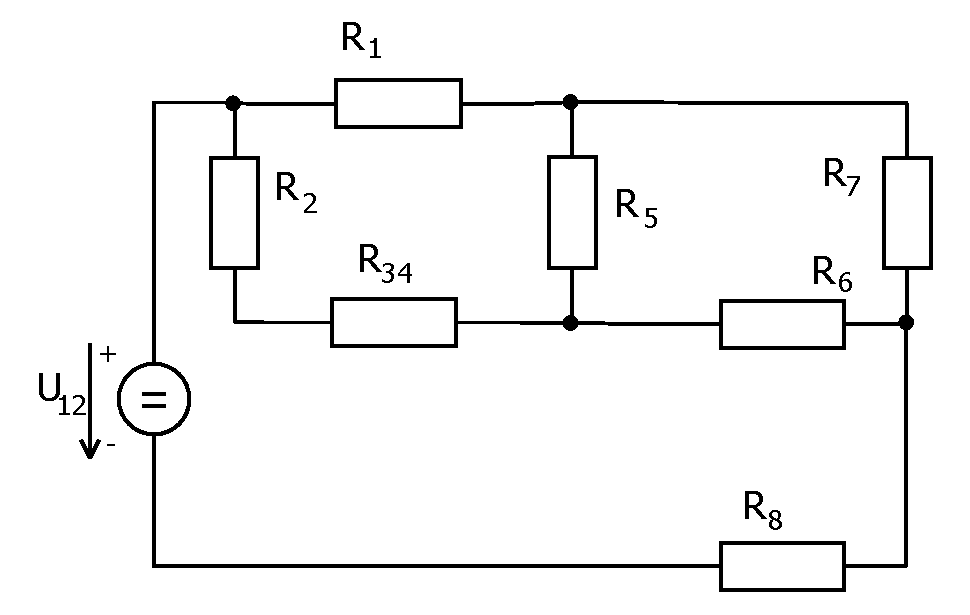
\includegraphics[width=0.6\linewidth]{obr/1_2}
		\caption{$R_3$ a $R_4$ jsou zapojeny paralelně a zdroje $U_1$ a $U_2$ sériově }
	\end{figure}
	\begin{gather*}
		R_{34} = \frac{R_3 R_4}{R_3 + R_4} =\frac{260 \cdot 310}{260 + 310} \doteq 141.4035 \Omega \\
		U_{12} = {U_1 + U_2} = {135 + 80} = 215  \text{V}
	\end{gather*}

	\begin{figure}[H]
		\center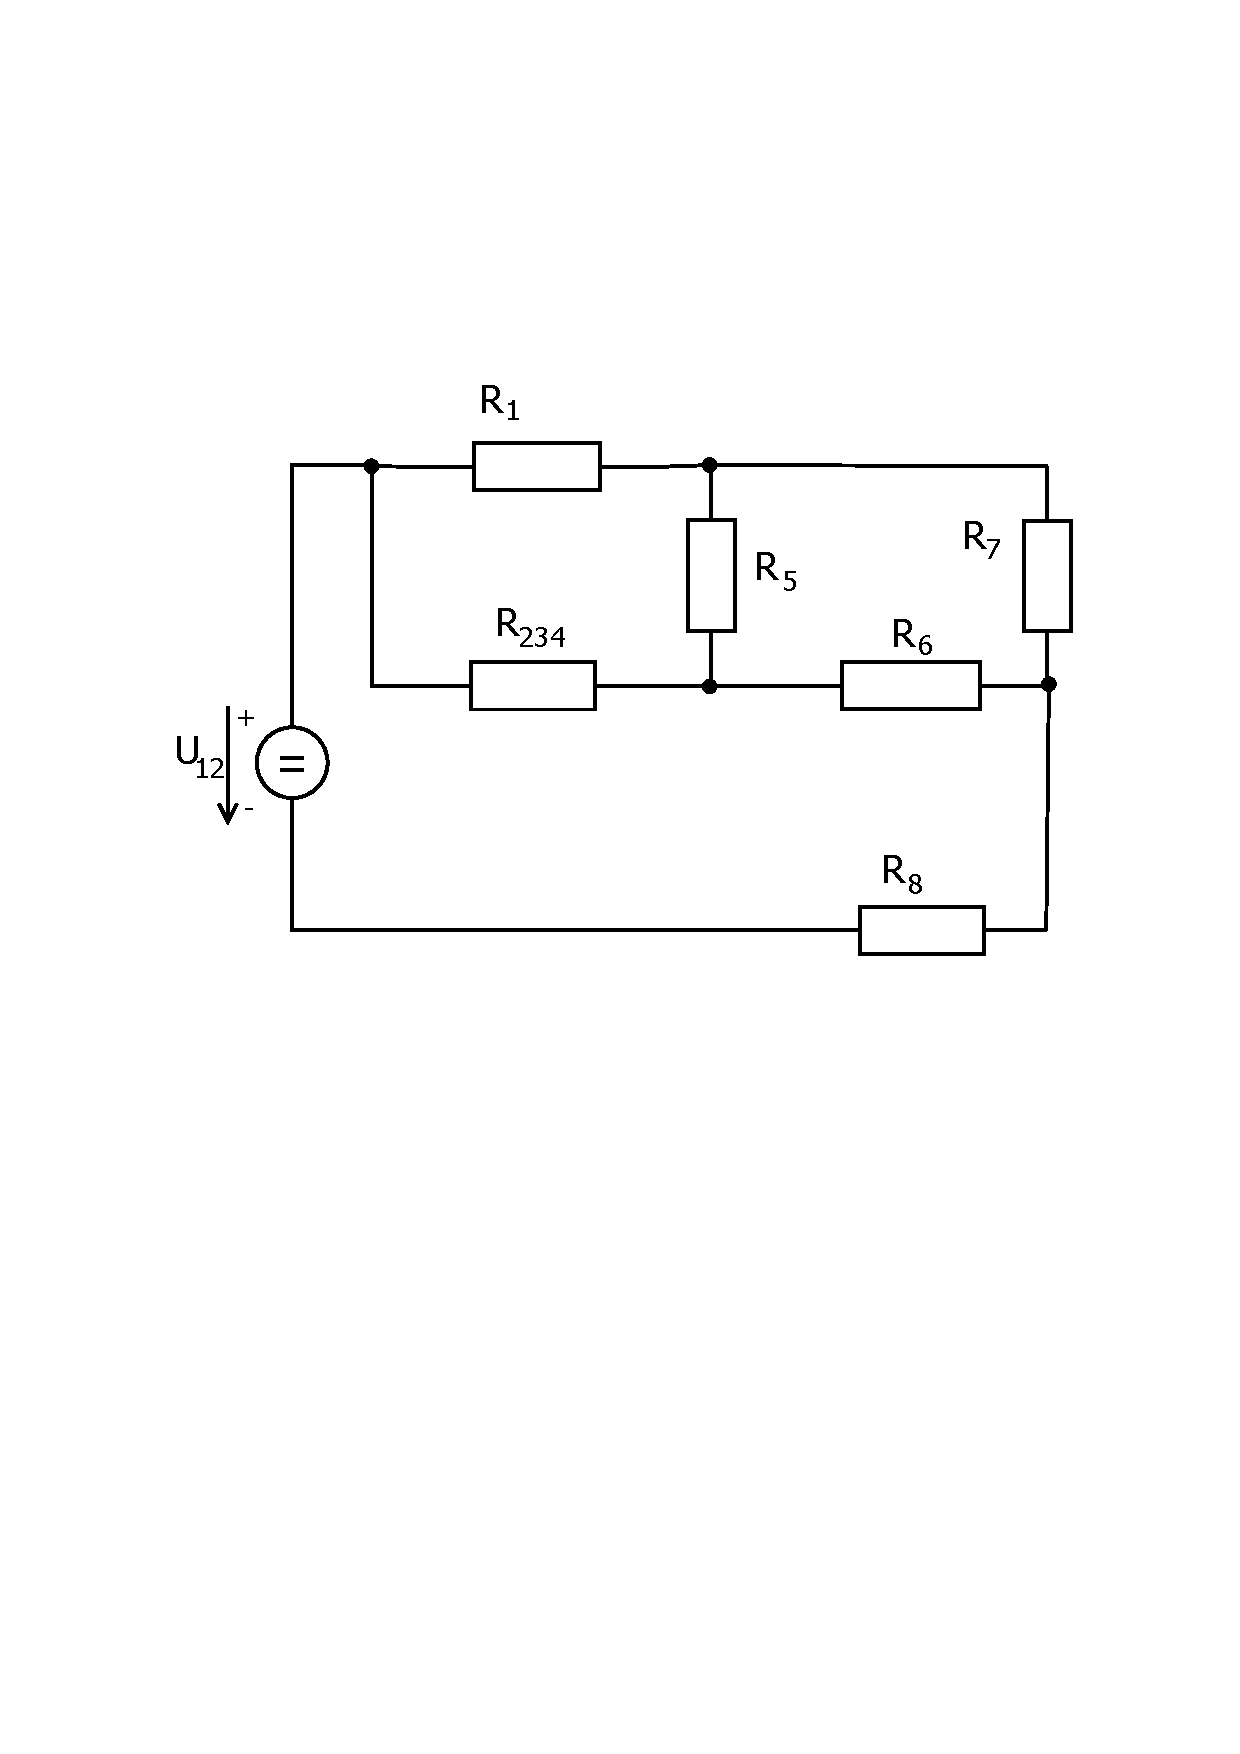
\includegraphics[width=0.6\linewidth]{obr/1_3}
		\caption{$R_2$ a $R_{34}$ jsou zapojeny sériově}
	\end{figure}
	\begin{gather*}
		R_{234} = R_2 + R_{34} = 600 + 140.4035 = 740,4035 \Omega
		\\
	\end{gather*}
	
	\begin{figure}[H]
		\vspace{-1.1cm}
		\center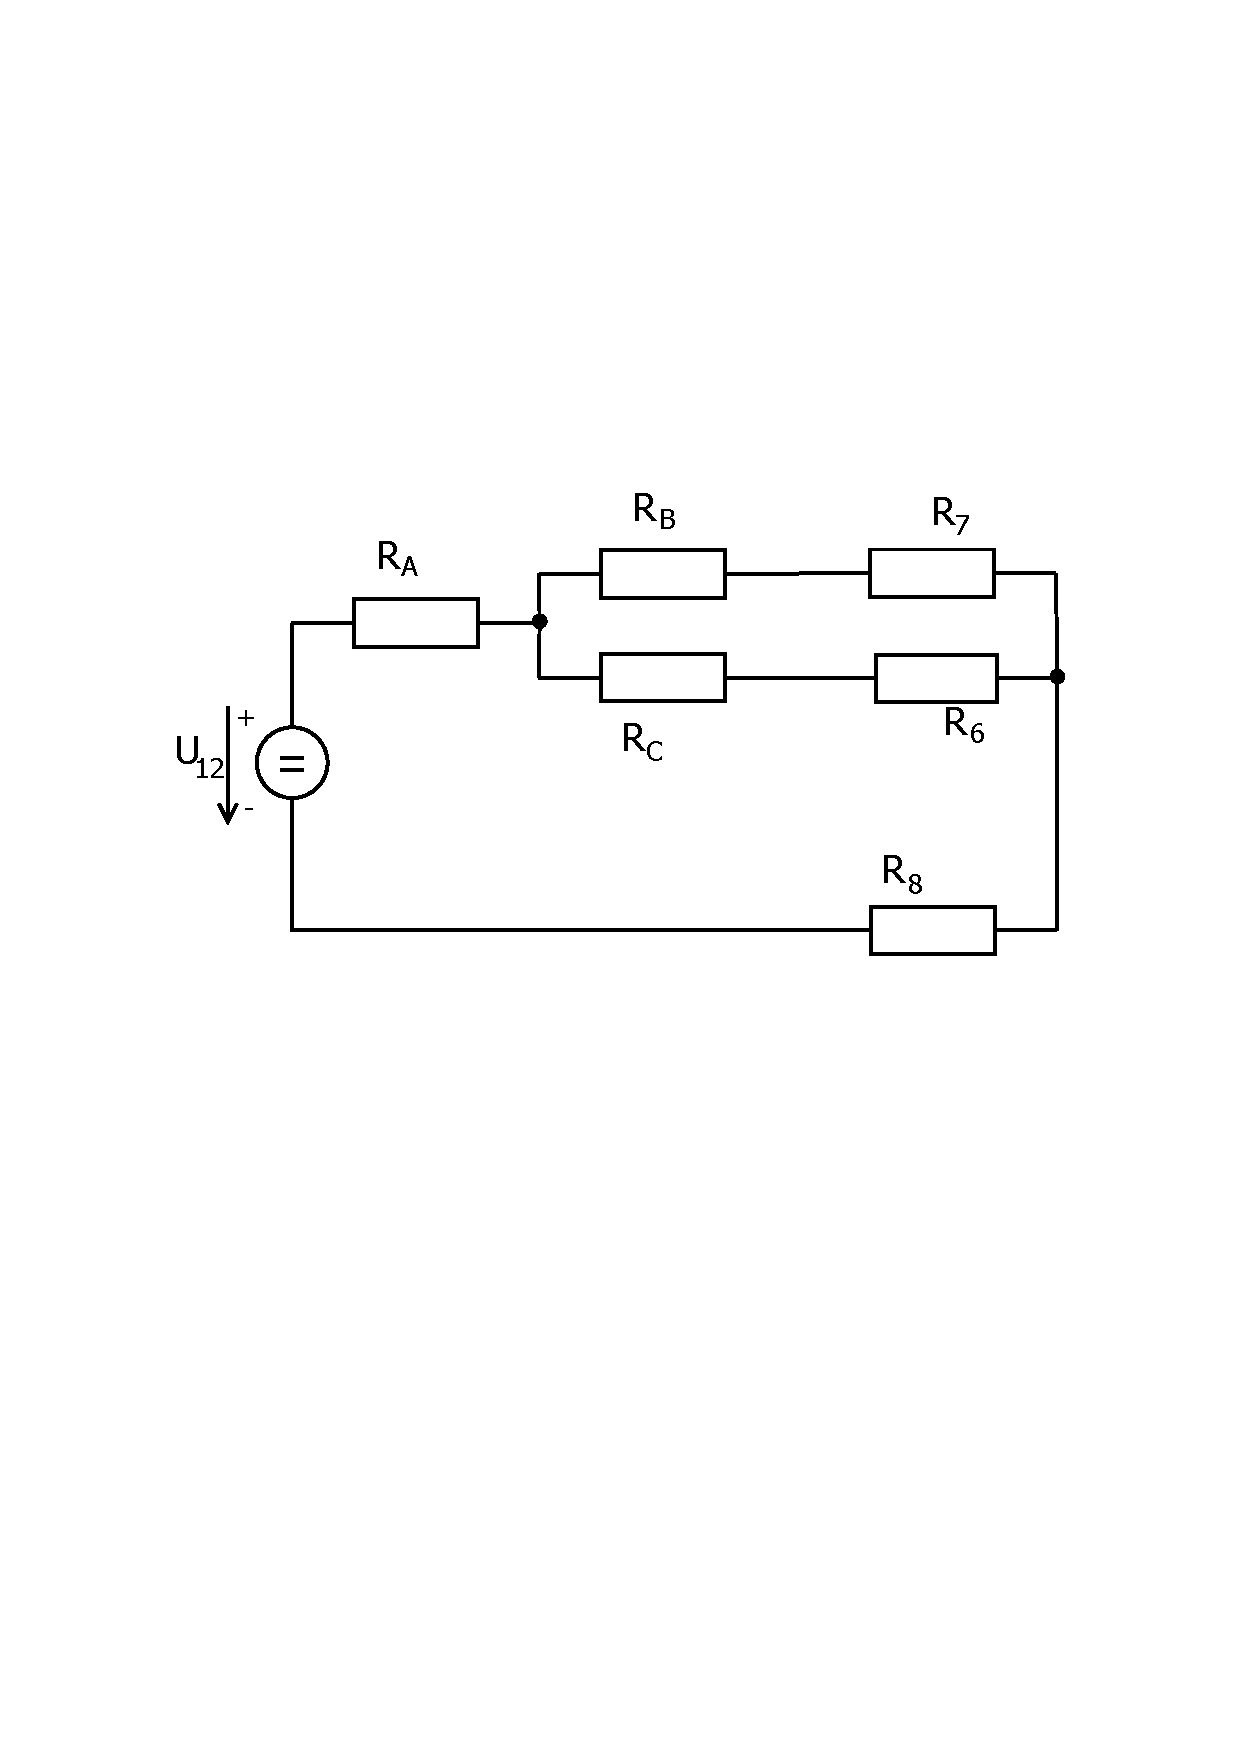
\includegraphics[width=0.6\linewidth]{obr/1_4}
		\caption{transfigurace - trojúhelník}
	\end{figure}
	\begin{gather*}
		R_A = \frac{R_1  R_{234}}{R_1 + R_{234} + R_5} = \frac{680 \cdot 740.4035}{680 +  740.4035 + 575} = 252.3171 \Omega \\
		R_B = \frac{R_1  R_5}{R_1 + R_{234} + R_5} = \frac{680 \cdot 575}{680 +  740.4035 + 575} = 195.9503 \Omega \\
		R_C = \frac{R_5  R_{234}}{R_1 + R_{234} + R_5} = \frac{575 \cdot 740.4035}{680 +  740.4035 + 575} = 213.3564 \Omega 
	\end{gather*}

	\begin{figure}[H]
		\center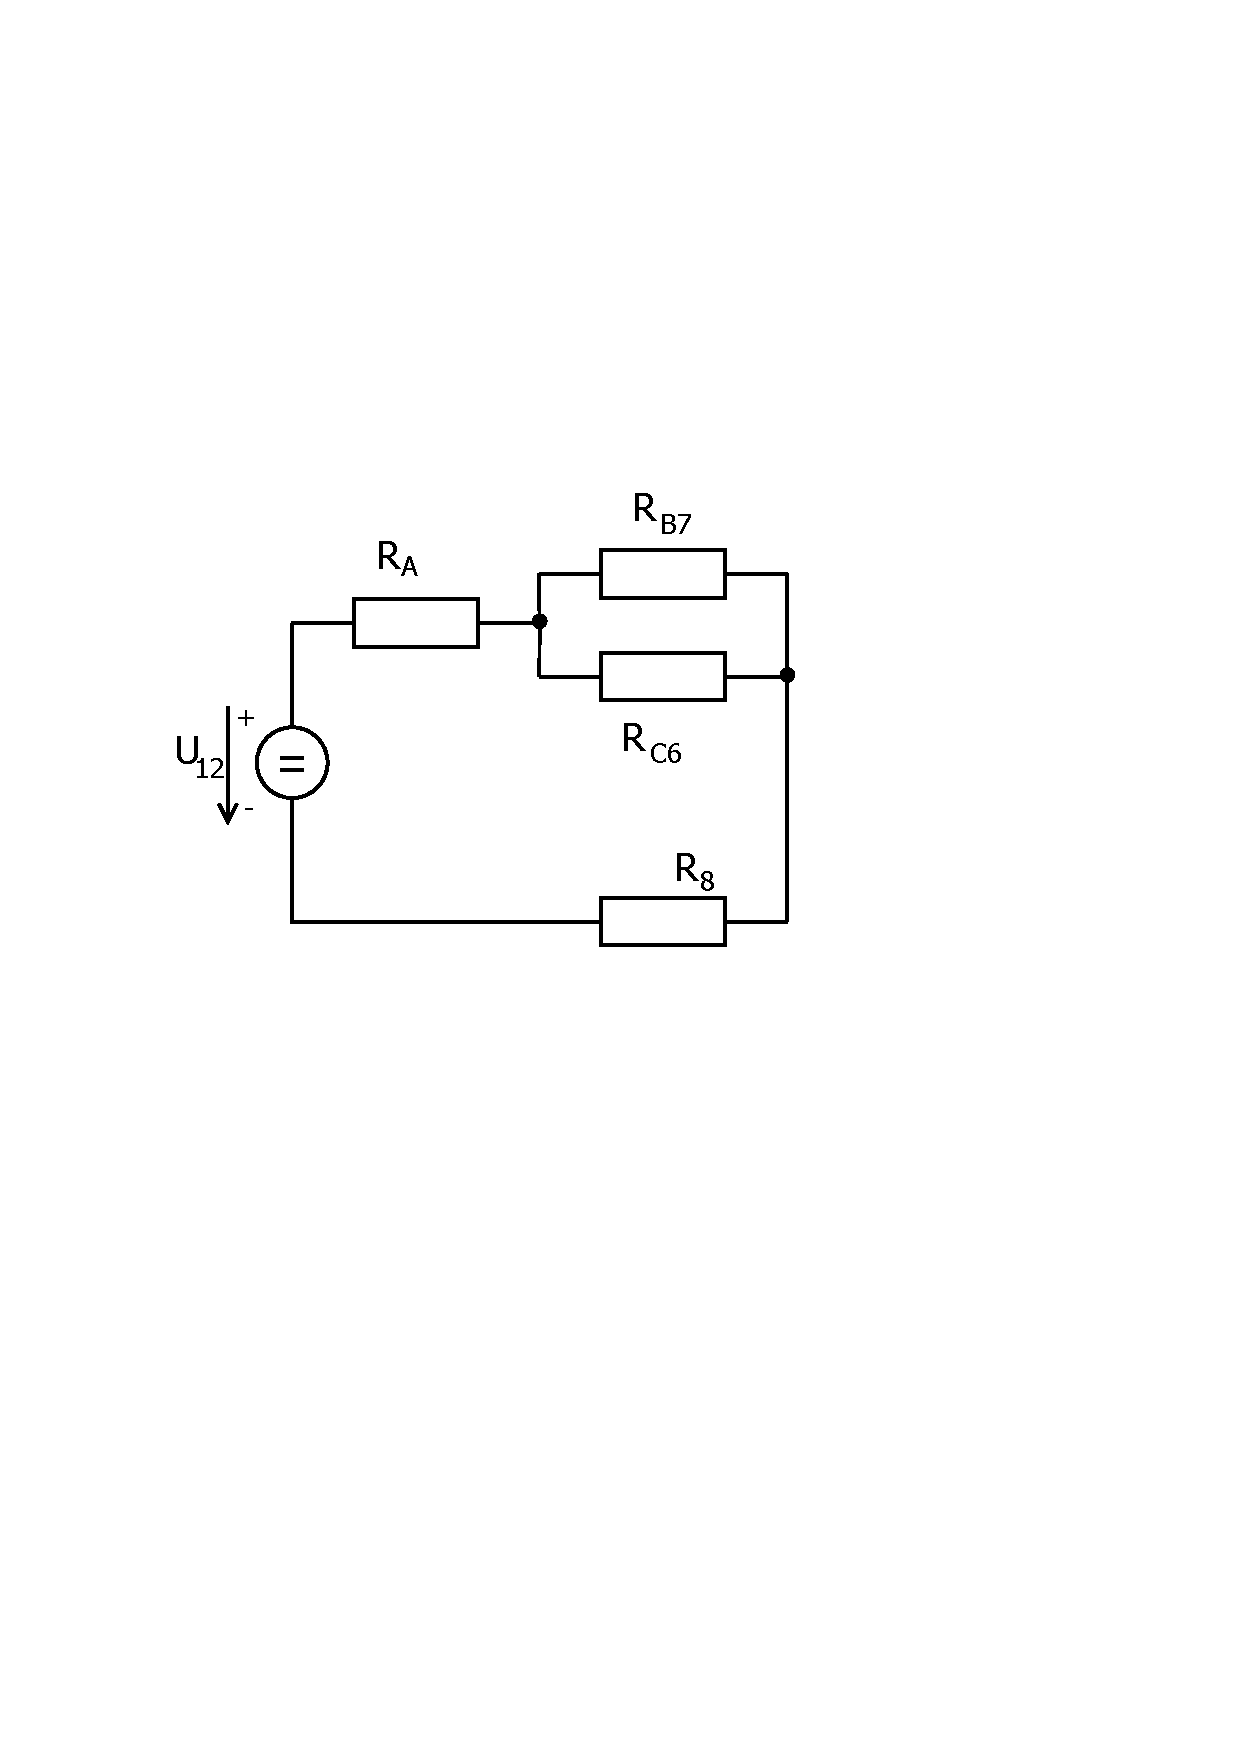
\includegraphics[width=0.6\linewidth]{obr/1_5}
		\caption{$R_B$ a $R_7$ jsou zapojeny sériově stejně jako $R_C$ a $R_6$}
	\end{figure}
	\begin{gather*}
		R_{B7} = R_B + R_7 = 195.9503 + 355 = 550.9503 \Omega \\
		R_{C6} = R_C + R_6 = 213.3564 + 870 = 1 083.3564 \Omega
	\end{gather*}


	\begin{figure}[H]
		\center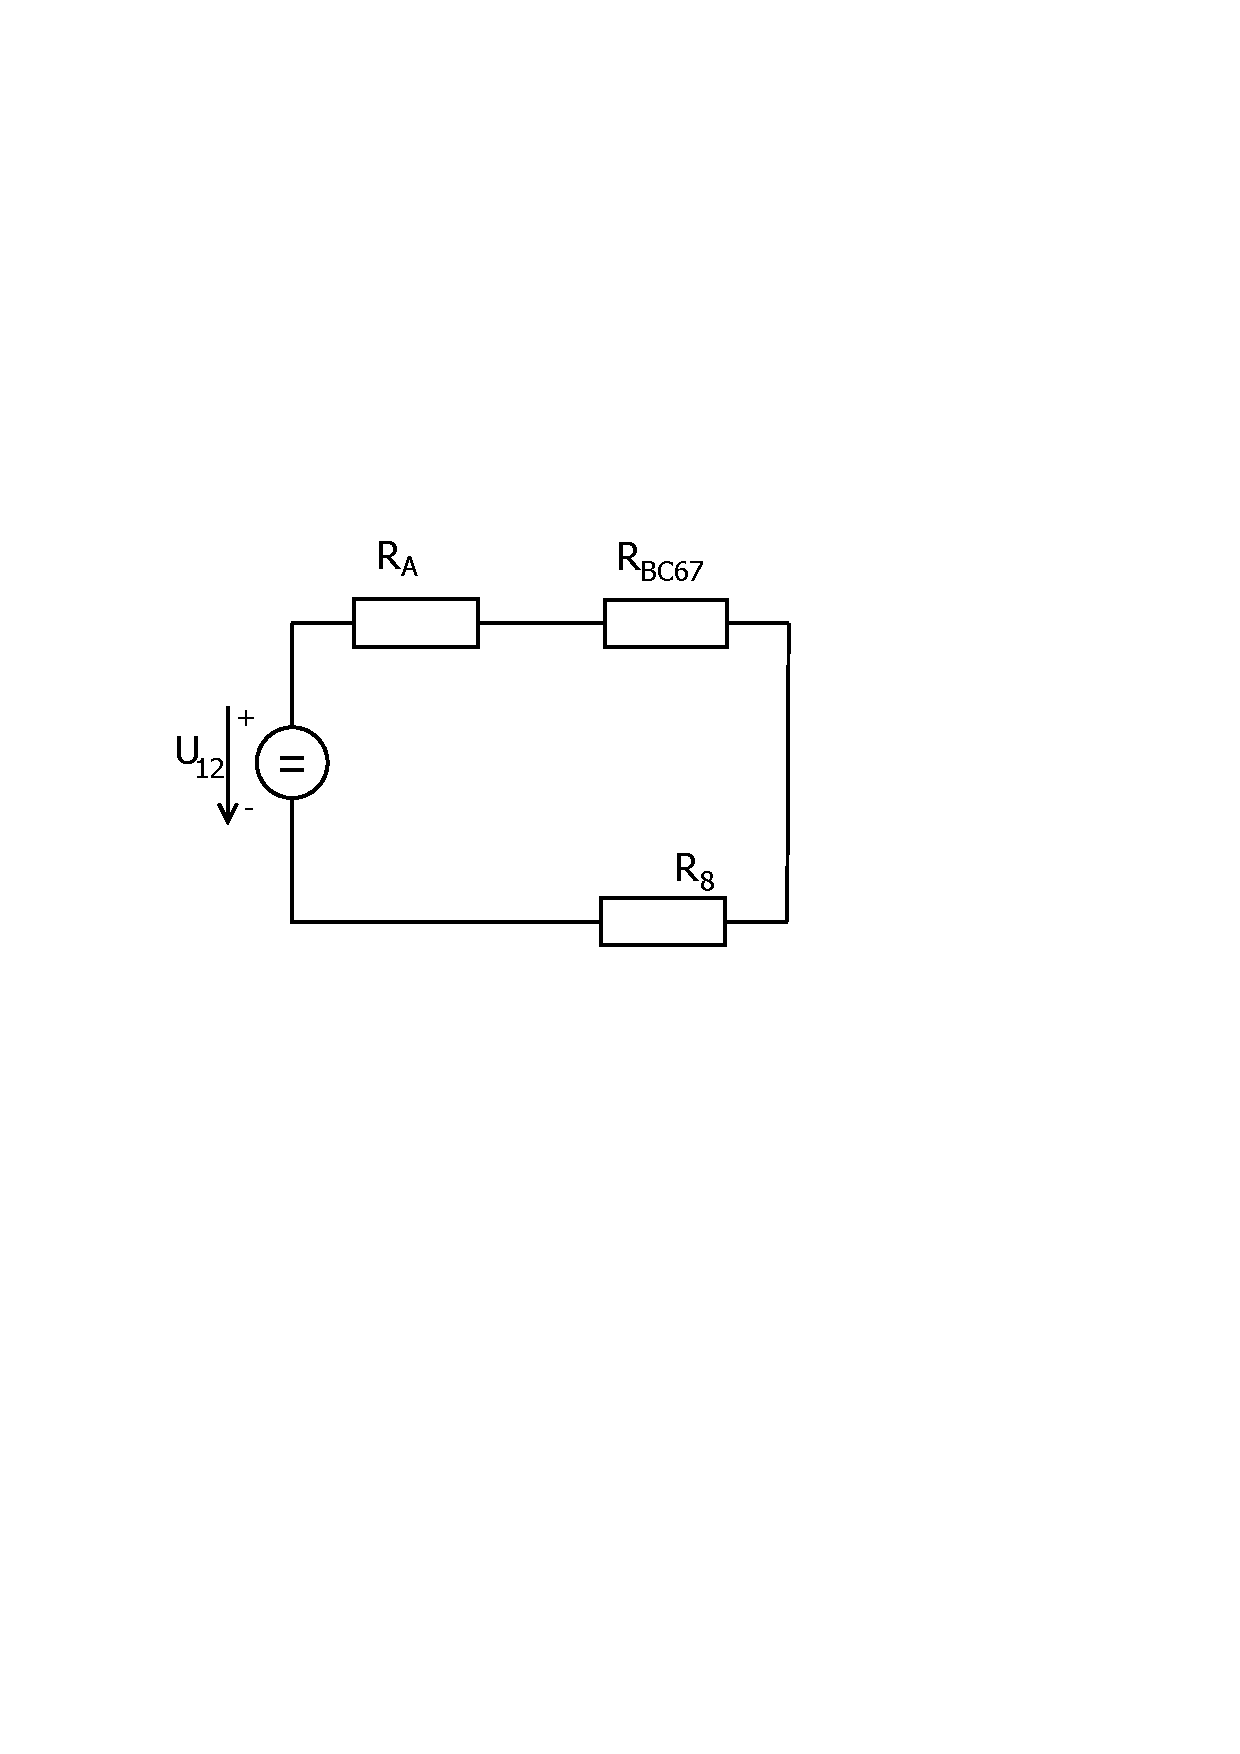
\includegraphics[width=0.6\linewidth]{obr/1_6}
		\caption{ $R_{B7}$ a $R_{C6}$ jsou zapojeny paralelně}
	\end{figure}
	\begin{gather*}
		R_{BC67} = \frac{R_{B7} R_{C6}}{R_{B7} + R_{C6}} = \frac{550.9503 \cdot 1 083.3564}{550.9503 + 1 083.3564} = 365.2163 \Omega
	\end{gather*}

	\begin{figure}[H]
		\center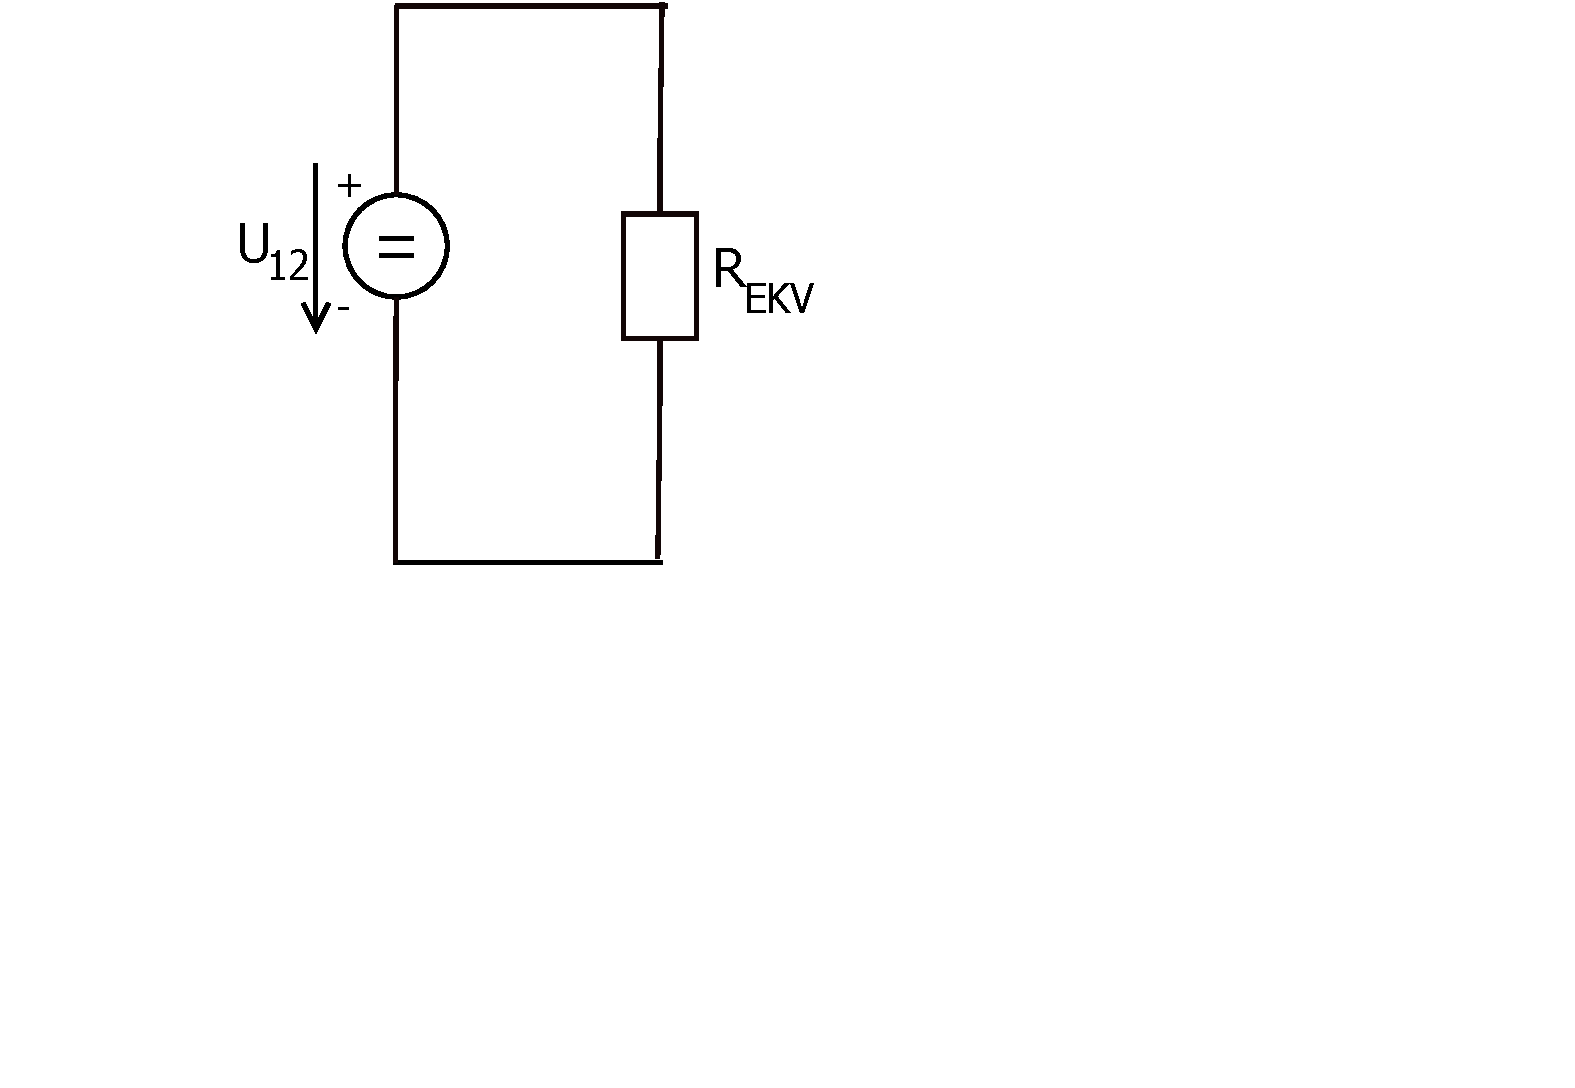
\includegraphics[width=0.3\linewidth]{obr/1_7}
		\caption{$R_A$ a $R_{BC67}$ a $R_8$ jsou zapojeny sériově - získáváme $R_{EKV}$}
	\end{figure}
	\begin{gather*}
		R_{EKV} = R_{A} + R_{BC67} + R_8 = 252.3171 + 365.2163 + 265 = 882.5334 \Omega
	\end{gather*}

	Celkový proud $I$:
	\begin{gather*}
		I = \frac{U_{12}}{R_{EKV}} = \frac{215}{882.5334} \doteq 0.2436 \text{A}
	\end{gather*}

	Začneme zpětně počítat napětí a proudy, až dojdeme k $U_{R_6}$ a $I_{R_6}$:

	\begin{figure}[H]
		\center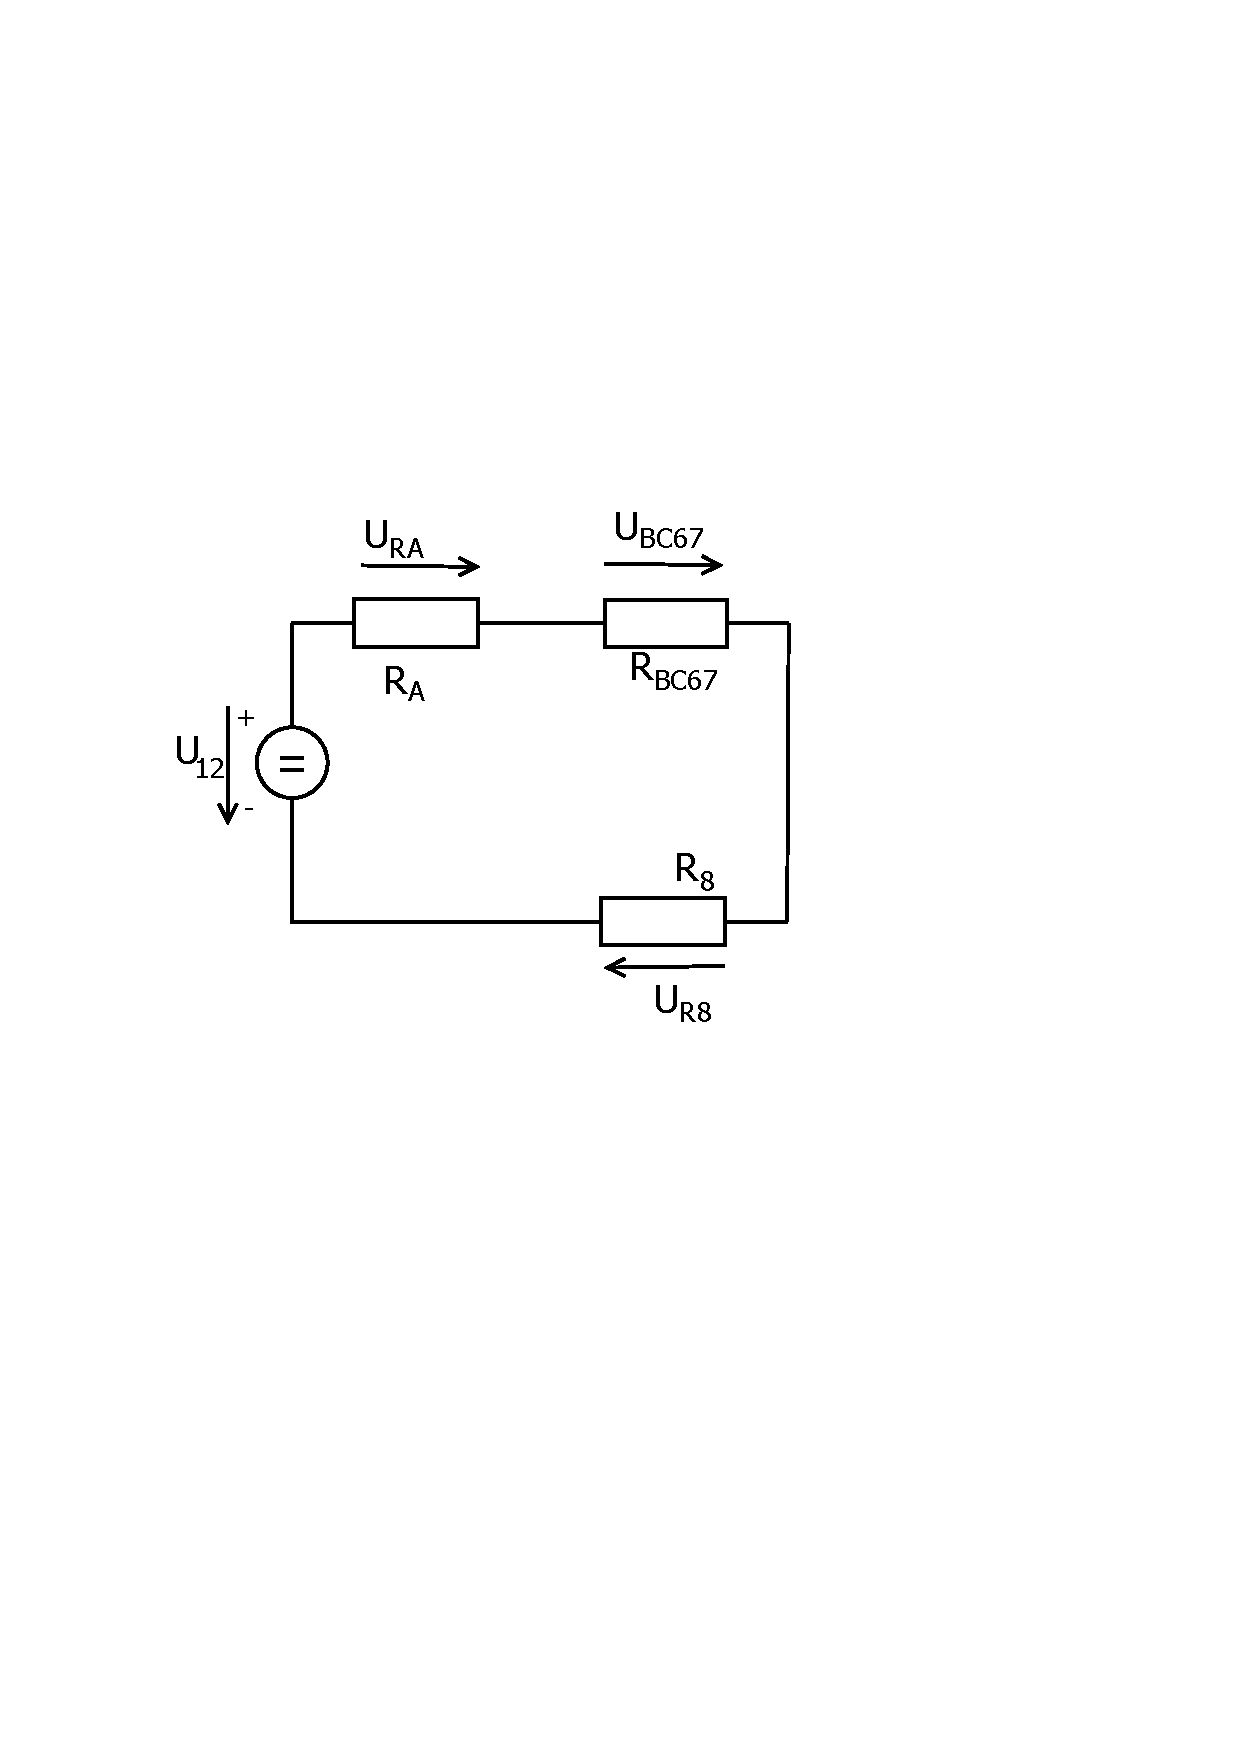
\includegraphics[width=0.6\linewidth]{obr/1_8}
		\caption{Spočítáme si napětí na jednotlivých odporech}
	\end{figure}
	\begin{gather*}
		U_{R_A} = {I R_A} = {0.2436\cdot 252.3171} \doteq 61.4644 \text{V} \\
		U_{R_{BC67}} = {I R_{BC67}} = {0.2436 \cdot 365.2163} \doteq 88.9667  \text{V} \\
		U_{R_8} = {I R_8} = {0.2436 \cdot 265} = 64.554  \text{V} \\
		\\
		\text{Provedeme kontrolu pomocí II. Kirchhoffova zákona.}  \\
		U_{R_A} + U_{R_{BC67}} + U_{R_8} - U_{12} =  0 \\
	\end{gather*}

	\begin{figure}[H]
		\center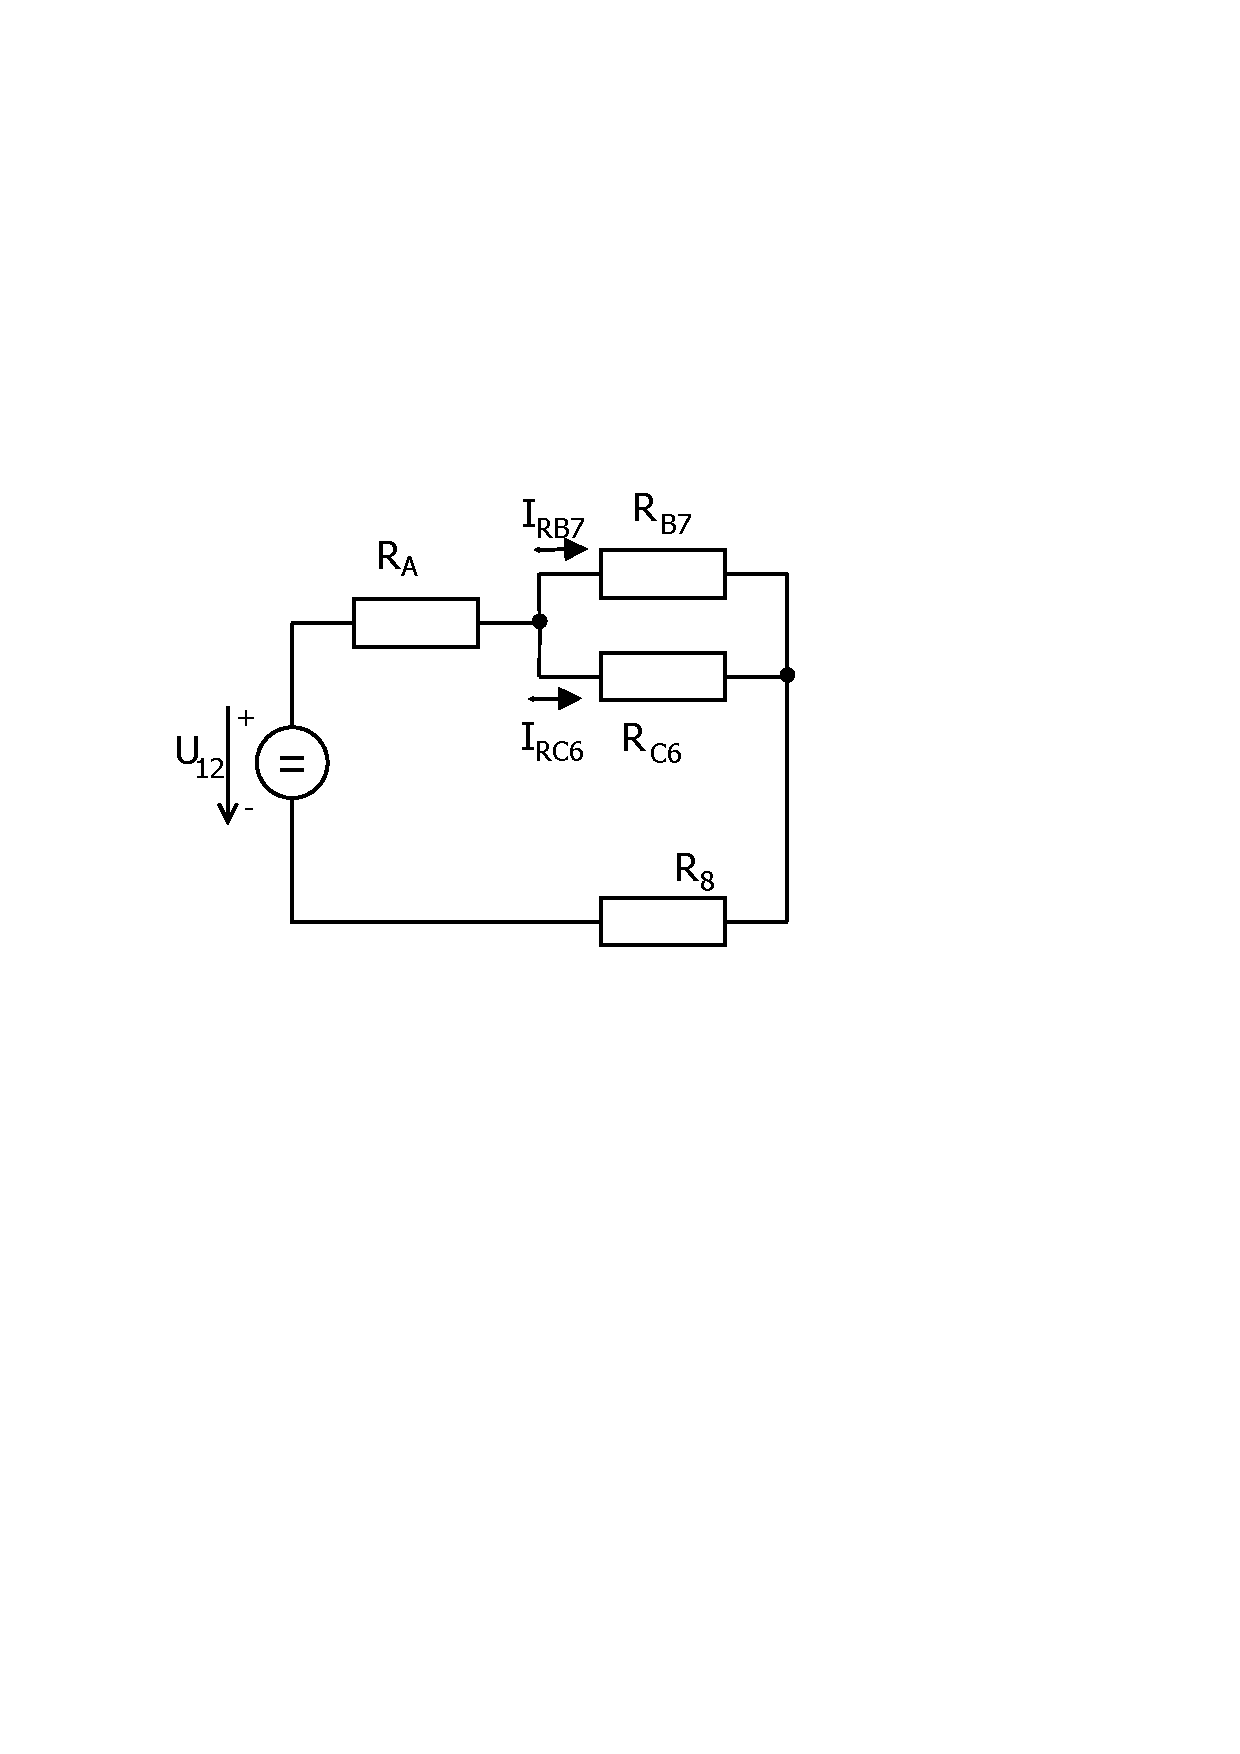
\includegraphics[width=0.6\linewidth]{obr/1_9}
		\caption{Spočítáme si proud ve větvích s $R_{B7}$ a  $R_{C6}$}
	\end{figure}
	\begin{gather*}
		I_{R_{B7}} = \frac{U_{R_{BC67}}}{R_{B7}} = \frac{88.9667}{550.9503} \doteq 0.1615 \text{A} \\
		I_{R_{C6}} = \frac{U_{R_{BC67}}}{R_{C6}} = \frac{88.9667}{1083.3564} \doteq 0.0821 \text{A} \\
		\\
		\text{Provedeme kontrolu pomocí I. Kirchhoffova zákona.}  \\
		I_{R_{B7}} + I_{R_{C6}} - I  =  0 
	\end{gather*}

	\begin{figure}[H]
		\center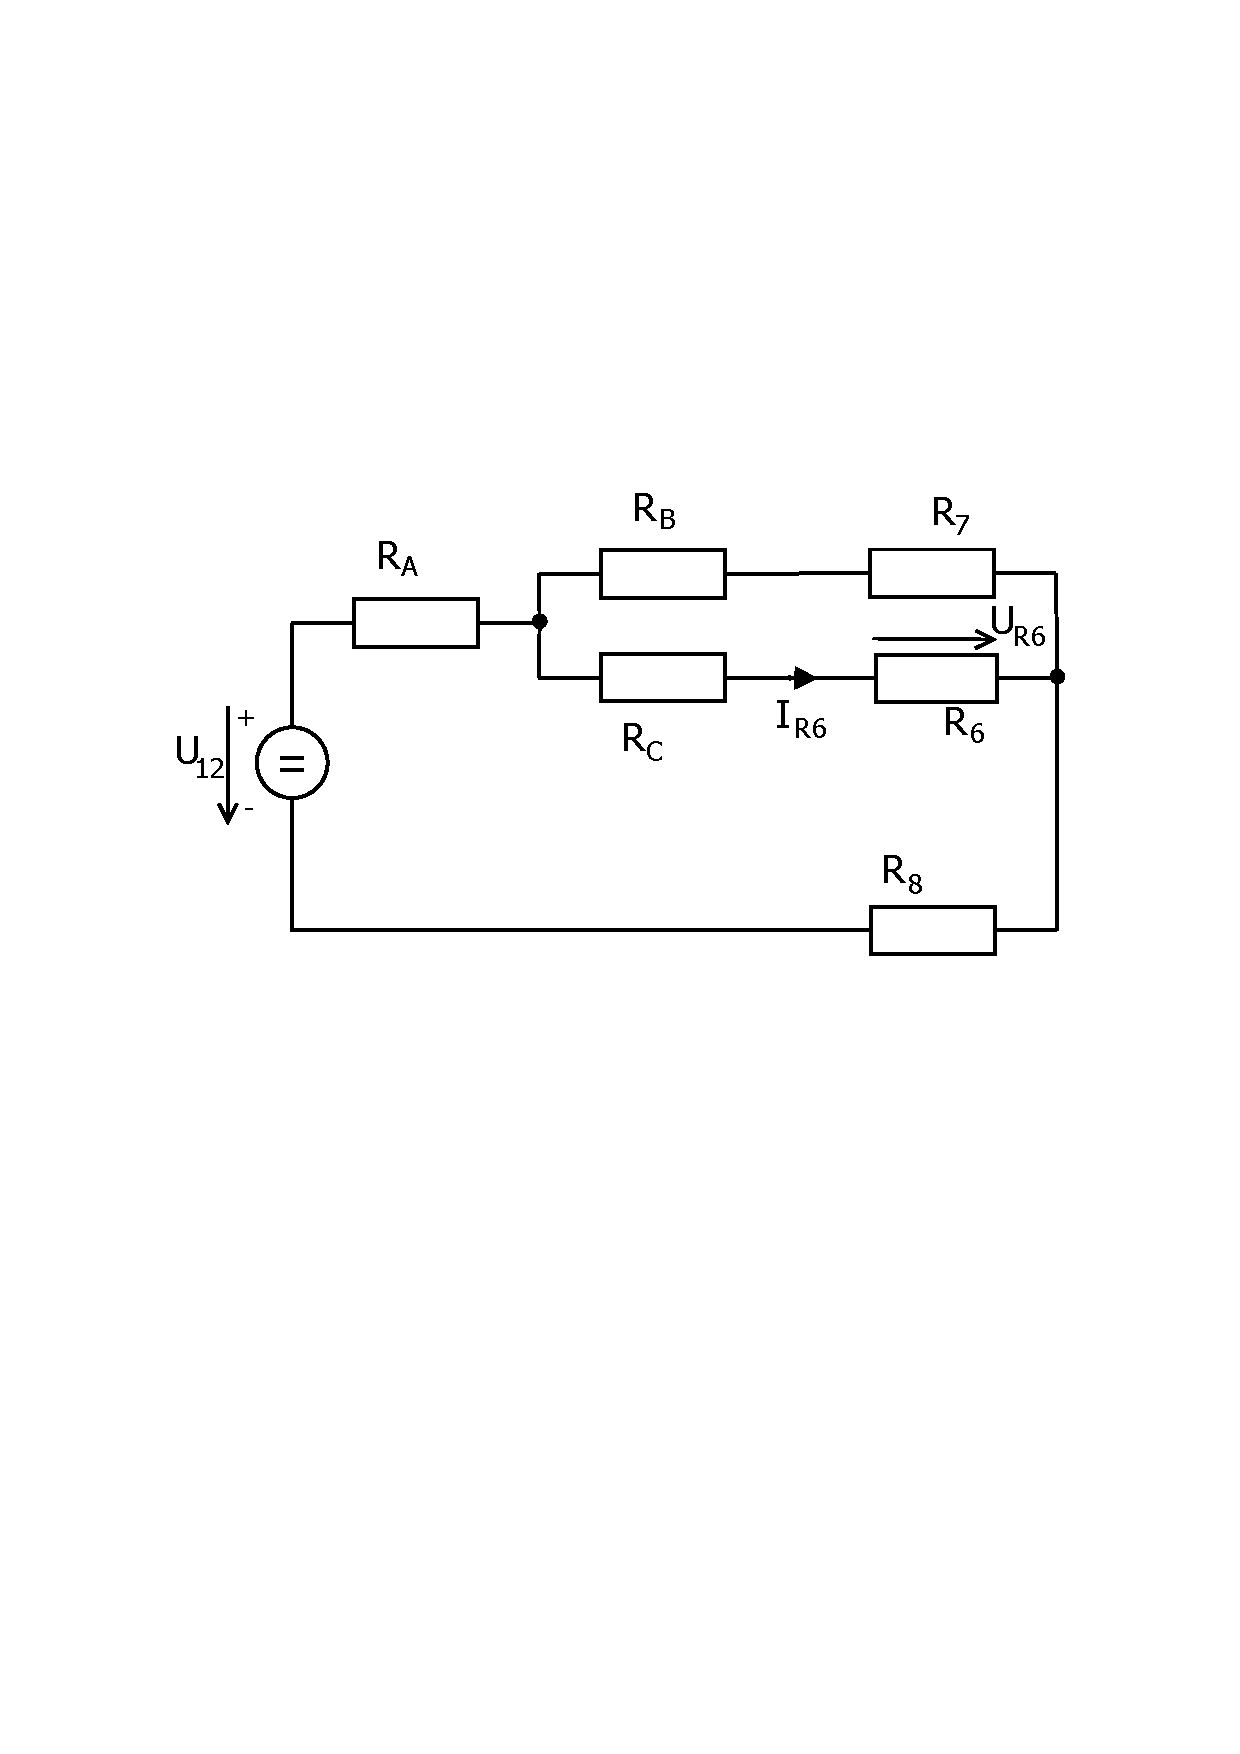
\includegraphics[width=0.6\linewidth]{obr/1_10}
		\caption{Spočítáme si napětí a proud u $R_6$}
	\end{figure}
	\begin{gather*}
		I_{R_{C6}} = I_{R_6} = 0.0821 \text{A} \\
		U_{R_6} = {I_{R_6} R_6} = {0.0821 \cdot 870} = 71.427  \text{V} \\
	\end{gather*}
	